


\chapter{TPM Hardware-Architektur}
\section{Einleitung}

Das TPM ist eine passive Chipkartenkomponente, die mit ihrem Benutzerstack gemäß einem Challenge-Response-Modell interagiert. Die Komponente ist vorzugsweise mit der Hauptplatine verlötet und hat einen bidirektionalen Zugriff auf die CPU.
Der Zugriff erfolgt über einen Low-Speed-LPC-Port mit einer Bandbreite von 256 MB / s und 1 GB / s je nach Modell, verwaltet von "South Bridge". Das TPM besteht aus mehreren Modulen, die in den folgenden Abschnitten funktional beschrieben werden.
Diese Klausel beschreibt den Gesamtbetrieb des TPM und die für seinen Betrieb erforderlichen Funktionseinheiten. Die Hauptelemente der Architektur sind in Abbildung 1 dargestellt.


\begin{figure}[h]
   
\begin{center}
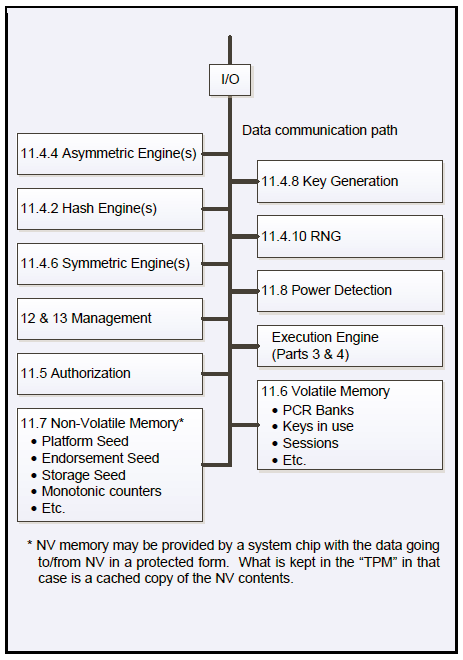
\includegraphics[scale=1]{Abbildung1.PNG} 
\captionof{figure}{Die Hauptelemente der TPM-Architektur}
\label{fig:strukturvorlage}
\label{fig1}

\end{center}

\end{figure}

\clearpage
\newpage

\section{Modul (I / O)}
Der I/O-Puffer ist der Kommunikationsbereich zwischen einem TPM und dem Hostsystem. Das System platziert Befehlsdaten in den I/O-Puffer und ruft Antwortdaten aus dem Puffer ab.
Eine Beschreibung der physischen Prozesse, die zum Verschieben von I/O-Pufferdaten zum / vom System verwendet werden, liegt außerhalb des Umfangs dieser Spezifikation. Plattformspezifische Arbeitsgruppen innerhalb der TCG erstellen auf ihren Plattformen die Spezifikationen für die physikalischen Schnittstellen zum TPM. Diese Spezifikationen beschreiben die Wechselwirkungen zwischen der Systemsoftware und dem TPM-I/O-Puffer.
Es ist nicht erforderlich, dass der I/O-Puffer physisch von anderen Teilen des Systems isoliert wird. Es kann sich um einen gemeinsam genutzten Speicher handeln. Wenn jedoch die Verarbeitung eines Befehls beginnt, muss die Implementierung sicherstellen, dass das TPM die richtigen Werte verwendet. Wenn das TPM beispielsweise als Teil der Berechtigungsverarbeitung einen Hash der Befehlsdaten ausführt, muss das TPM die validierten Befehlsdaten vor der Änderung schützen. Das heißt, bevor die Daten validiert werden, müssen sie vor Änderungen geschützt werden. Bevor die Daten geändert werden, müssen sie sich an einem abgeschirmten Ort befinden.

\section{Kryptographie-Subsystem}
\subsection{Einleitung}
Das Cryptography-Subsystem implementiert die kryptografischen Funktionen des TPM. Es kann vom Befehlsparsemodul, vom Autorisierungssubsystem oder vom Befehlsausführungsmodul aufgerufen werden. Das TPM verwendet konventionelle kryptographische Operationen auf konventionelle Weise. Diese Operationen umfassen : \\
• Hashfunktionen,  \\
• asymmetrische Ver- und Entschlüsselung \\
• asymmetrische Signatur und Signaturprüfung \\
• symmetrische Ver- und Entschlüsselung \\
• Symmetric Signing (HMAC) und Signaturprüfung sowie \\
• Schlüsselerzeugung. \\
Der Rest dieser Klausel beschreibt einige Algorithmen, die normalerweise in einem TPM gefunden werden, um zu zeigen, wie sie gehandhabt werden. Diese Beschreibungen veranschaulichen die Auswahl verfügbarer Algorithmen, schränken sie jedoch nicht ein.
\subsection{Hash-Funktionen}
Hash-Funktionen können direkt von externer Software oder als Nebeneffekt vieler TPM-Vorgänge verwendet werden. Das TPM verwendet Hashing, um die Integritätsprüfung und Authentifizierung sowie bei Bedarf Einwegfunktionen (sowie KDF) bereitzustellen.
Ein TPM sollte einen genehmigten Hash-Algorithmus implementieren, der ungefähr die gleiche Sicherheitsstärke wie sein stärkster asymmetrischer Algorithmus aufweist.
\\  \\ \\
Zum Beispiel : 
Ein ECC mit einem 384-Bit-Schlüssel hat eine Sicherheitsstärke von 192 Bit. SHA384 mit 192 Bit Sicherheit würde die obige Anforderung erfüllen.
\\ \\
Eine Hash-Funktion wird durch Halgorithm () bezeichnet, wobei der Algorithmus-Index den Hash-Algorithmus oder den Parameter angibt, der den Hash-Algorithmus-Bezeichner enthält. In einigen Fällen fehlt der Algorithmus-Index. In diesem Fall wird der Algorithmus durch den Kontext bestimmt.
Das Command Dispatch-Modul verwendet die Hash-Funktion, um bestimmte Arten von Berechtigungen zu überprüfen. Hash-Funktionen werden auch zur Unterstützung anderer Operationen im TPM wie PCR Extend verwendet.

\subsection{HMAC-Algorithmus}

Dieses Modul implementiert die Schlüsselhash-Funktion HMAC. Die Größe der Schlüssel beträgt 20 Byte und die Größe der Blöcke beträgt 64 Byte.
Die Funktion unterstützt die Berechnung von HMAC nach RFC 2104. \\
Das TPM implementiert den in ISO / IEC 9797-2 beschriebenen Algorithmus für den Hash Message Authentication Code (HMAC).
Ein HMAC ist eine Form der symmetrischen Signatur einiger Daten. Sie bietet die Sicherheit, dass geschützte Daten nicht geändert wurden und von einer Entität mit Zugriff auf einen Schlüsselwert stammen. Der Schlüsselwert muss ein Geheimnis oder ein gemeinsames Geheimnis sein, um Daten schützen zu können. \\
Das Command Dispatch-Modul kann die HMAC-Funktion verwenden, um eine Autorisierung zu überprüfen. Die HMAC-Funktion kann vom Befehlsausführungsmodul zur Unterstützung seiner Operationen verwendet werden.

\subsection{Asymmetrische Operationen}

Ein TPM verwendet asymmetrische Algorithmen für die Bestätigung, Identifizierung und das Teilen von geheimen Daten. Ein TPM kann jeden asymmetrischen Algorithmus unterstützen, dem die TCG eine Kennung zugewiesen hat. Ein asymmetrischer Algorithmus-Identifikator zeigt eine Familie von Algorithmen und Methoden an, die mit diesem Algorithmus verwendet werden.
Die Methoden zur Verwendung eines asymmetrischen Algorithmus finden Sie in algorithmischen Anhängen zu diesem TPM 2.0, Teil 1. Derzeit werden die einzigen unterstützten asymmetrischen Algorithmen RSA (in Anhang B beschrieben) und ECC mit Primerkurven (in Anhang B beschrieben).
Ein TPM ist erforderlich, um mindestens einen asymmetrischen Algorithmus zu implementieren.

\subsection{Signaturoperationen}
\subsubsection{Signierung}
Das TPM kann entweder mit einem asymmetrischen oder einem symmetrischen Algorithmus signieren. Die Art der Signatur hängt von der Art des Schlüssels ab. Bei einem asymmetrischen Algorithmus hängen die Signiermethoden vom Algorithmus (RSA oder ECC) ab. Für symmetrische Signaturen ist derzeit nur das HMAC-Signaturschema definiert. Wenn ein Schlüssel zum Signieren verwendet werden kann, hat er das Zeichenattribut.
\\
Ein Schlüssel mit einem Zeichenattribut kann auch eine Einschränkung für den Inhalt der Nachricht haben, die mit dem Schlüssel signiert werden kann. Wenn für einen Schlüssel diese Einschränkung gilt, verwendet das TPM den Schlüssel nicht zum Signieren von Nachrichtenauszügen, die das TPM nicht berechnet hat.
\\
Jede von einem TPM erzeugte Attestierungsnachricht verfügt über einen Header (TPM\_GENERATED\_VALUE), um die Daten als innerhalb eines TPM erzeugte Daten zu identifizieren. Wenn ein eingeschränkter Schlüssel zum Signieren dieser Daten verwendet wird, kann sich eine vertrauende Partei darauf verlassen, dass die Nachrichtendaten von einem TPM stammen.
\\
Damit ein eingeschränkter Schlüssel eine extern generierte Nachricht signieren kann, wird das TPM zur Erstellung des Message Digest verwendet. Wenn das TPM den Digest berechnet, überprüft es, dass die Nachricht nicht mit TPM\_GENERATED\_VALUE beginnt. Wenn dies der Fall ist, erstellt das TPM keine spezielle Zertifizierung (ein Ticket), die angibt, dass der Digest vom TPM erstellt wurde und mit einem eingeschränkten Schlüssel sicher signiert werden kann.
\\
Ein als Signaturschlüssel bezeichneter Schlüssel kann in jedem Befehl verwendet werden, der einen Signaturschlüssel verwendet. Für einige Befehle kann das Signaturschema im Befehl angegeben werden. Nicht alle Schemas gelten für alle Schlüssel. Das TPM generiert einen Fehler, wenn das Schema mit dem angegebenen Schlüsseltyp nicht zulässig ist.
\\
Zum Beispiel 1 : Das RSASSA-PKCS1-v1\_5-Signaturschema ist bei einem ECC-Schlüssel nicht gültig.
\\
Zum Beispiel 2 : Ein Schlüssel mit dem Attribut "eingeschränkt" darf nur mit einem Signaturschema verwendet werden. Wenn es für die Verwendung mit RSASSA-PSS beschränkt ist, kann es nicht mit RSASSA\-PKCS1\-v1\_5 verwendet werden.
\\
Ein eingeschränkter Signaturschlüssel ist erforderlich, damit in der Schlüsseldefinition ein Signaturschema angegeben wird, das das einzige Signaturschema ist, das mit dem Schlüssel verwendet werden darf. Bei einem uneingeschränkten Schlüssel kann die Schlüsseldefinition eine Auswahl eines Signaturschemas enthalten, oder das Signaturschema kann bestimmt werden, wenn der Schlüssel verwendet wird. Um die Auswahl des Signaturschemas zu verschieben, wird der Schlüssel mit TPM \_ALG\_NULL als Signaturschemaauswahl erstellt.
\subsubsection{Signaturprüfung}
TPM2\_VerifySignature () validiert eine Signatur. Der Befehl verwendet einen öffentlichen Schlüssel, einen Digest und einen Block, der die Signatur über dem Digest enthält.
Das TPM überprüft, ob das Signaturschema mit dem ausgewählten Schlüssel kompatibel ist. Jede Kombination von Hashes und nicht anonymen Signaturschemata, die ein TPM zum Signieren unterstützt, wird auch für die Signaturprüfung unterstützt.
Wenn die Signatur gültig ist, erstellt das TPM ein Ticket.
\subsubsection{Tickets}
Ein Ticket ist eine HMAC-Signatur, die einen Proof-Wert als HMAC-Schlüssel verwendet.
 \\
 Das TPM verwendet Tickets für zwei Zwecke:
 \\
 • Daten erneut signieren. Nach der Überprüfung einer asymmetrischen Signatur signiert das TPM den Digest mit einem symmetrischen TPM-Schlüssel erneut. Das TPM kann eine Signatur später erneut prüfen, ohne den asymmetrischen Schlüssel laden zu müssen.
 \\
 • Erweiterungsspeicher. Beim Hashing einer externen Nachricht hat das TPM einen Status, der angibt, dass die Nachricht nicht mit TPM\_GENERATED\_VALUE begann. Diese Statusinformationen können im TPM nicht unbegrenzt gespeichert werden. Mit einem Ticket kann dieser Status vom TPM auf eine Weise gespeichert werden, die für das TPM leicht zu überprüfen ist. Wenn dem TPM später ein Digest zum Signieren vorgelegt wird, wird das Ticket bereitgestellt, sodass das TPM überprüfen kann, dass das zu signierende Digest sicher signiert werden kann.
 \\
 Der für ein Ticket verwendete Proof-Wert hat minimal eine Anzahl von Bits, die der Größe des Digests entspricht, der vom Hash-Algorithmus erzeugt wird.
 \\
 Zum Beispiel :
Für ein SHA256-Ticket ist ein Korrekturwert von 256 Bit erforderlich.
\\
Es gibt fünf verschiedene Ticketarten:
\\
1) TPMT\_TK\_CREATION
\\
2) TPMT\_TK\_VERIFIED
\\
3) TPMT\_TK\_AUTH
\\
4) TPMT\_TK\_HASHCHECK
\\
5) NULL Ticket – A NULL
\\
\subsection{Symmetrische Verschlüsselung}
Das TPM verwendet die symmetrische Verschlüsselung, um einige Befehlsparameter (normalerweise Authentifizierungsinformationen) zu verschlüsseln und um außerhalb des Bereichs gespeicherte geschützte Objekte zu verschlüsseln. Der Cipher Feedback Mode (CFB) ist der einzige von dieser Spezifikation geforderte Block-Chipher-Modus.
\\
Jede von einem TPM unterstützte symmetrische Blockverschlüsselung kann zur Parameterverschlüsselung verwendet werden. Schwache Schlüssel dürfen jedoch nicht verwendet werden. Darüber hinaus sollte ein TPM die XOR-Verschleierung unterstützen, bei der es sich um eine Hash-basierte Stream-Verschlüsselung handelt. Die XOR-Verschleierung darf nur für die vertrauliche Parameterübergabe verwendet werden.
\\
Bei der Paarung mit einem asymmetrischen Schlüssel - wie bei einem ECC-Entschlüsselungsschlüssel - muss ein symmetrischer Schlüssel so viele Sicherheitsstärken aufweisen wie der asymmetrische Schlüssel, mit dem er gepaart wird.
\\
Zum Beispiel :
SP800\-57 klassifiziert 2048\-Bit\-RSA als 112-Bit-Sicherheit. AES mit 128\- oder 256\-Bit\-Schlüsseln bietet ausreichende symmetrische Sicherheit für das Pairing mit einem 2048\-Bit\-RSA\-Schlüssel.
\\ Wenn ein symmetrischer Schlüssel zur Datenverschlüsselung verwendet wird, haben die verschlüsselten Daten eine HMAC. Diese HMAC wird geprüft, bevor die Daten entschlüsselt werden. Durch die Überprüfung, dass die entschlüsselten Daten ordnungsgemäß mit dem symmetrischen Schlüssel verknüpft sind, wird die Leistungsanalyse schwieriger. Um den Schutz zu überwinden, wäre es notwendig, zwei verschiedene Schutzfamilien zu besiegen, anstatt einen zu haben, der vorhanden wäre, wenn der Integritätsschutz auf den Klartext und nicht auf den Chiffretext angewendet würde.
\\
\subsection{Schlüsselgenerierung}
Die Schlüsselerzeugung erzeugt zwei verschiedene Arten von Schlüsseln. Der erste, ein gewöhnlicher Schlüssel, wird unter Verwendung des Zufallszahlengenerators (RNG) erzeugt, um die Berechnung zu starten. Das Ergebnis der Berechnung ist ein geheimer Schlüsselwert, der an einem abgeschirmten Ort aufbewahrt wird.
\\
Der zweite Typ, ein Primärschlüssel, wird von einem Startwert abgeleitet, nicht direkt vom RNG. Der RNG erzeugt normalerweise den Samen, der dauerhaft im TPM gespeichert ist. Die Generierung eines Primärschlüssels aus einem Seed basiert auf der Verwendung einer genehmigten Schlüsselableitungsfunktion (KDF). Das KDF von SP800-108 wird in dieser Spezifikation häufig verwendet.
\\
Diese Spezifikation legt keine Obergrenze für die Zeit fest, die zum Generieren eines Schlüssels zulässig ist. Plattformspezifische Spezifikationen können die Zeit zum Generieren verschiedener Schlüsseltypen einschränken.
\\
Je nach Anwendung generiert das TPM möglicherweise einen Schlüssel durch :
\\
• Verwenden von Bits aus dem RNG oder \\
• Ableiten des Schlüssels von einem anderen geheimen Wert.


Es gibt viele Möglichkeiten, Schlüssel zu generieren. Diese Methoden werden in jeder Klausel ausführlich beschrieben, wo die Generierung eines Schlüssels erforderlich ist.

\subsection{Random Number Generator (RNG) Modul}
\subsubsection{Quelle der Zufälligkeit}
Der RNG ist die Quelle der Zufälligkeit im TPM. Das TPM verwendet Zufallswerte für Nonces, bei der Schlüsselerzeugung und für die Zufälligkeit von Signaturen.
Der RNG ist eine geschützte Fähigkeit ohne Zugangskontrolle. Es besteht nominell aus \\
• Eine Entropiequelle und einen Sammler, \\
• Ein staatliches Register, \\
• Eine Mischfunktion (typischerweise eine zugelassene Hash-Funktion). \\
Der Entropie-Kollektor sammelt Entropie aus Entropiequellen und entfernt Verzerrungen. Die gesammelte Entropie wird dann verwendet, um das Zustandsregister zu aktualisieren, das der Mischfunktion Input liefert, um die Zufallszahlen zu erzeugen. \\
Das RNG sollte die Zertifizierungsanforderungen des beabsichtigten Marktes erfüllen. \\
Das TPM sollte für jede Verwendung durch eine interne Funktion eine ausreichende Zufälligkeit bieten. Wenn auf sie durch einen externen Anruf zugegriffen wird, sollte sie in der Lage sein, 32 Oktette Zufälligkeit bereitzustellen. Größere Anfragen können fehlschlagen, wenn nicht genügend Zufälligkeit vorhanden ist. \\
Jeder RNG-Zugriff erzeugt einen neuen Wert, unabhängig von der Verwendung der Daten. Es wird nicht zwischen Zugriffen für interne und externe Zwecke unterschieden.

\subsubsection{Entropiequelle und Kollektor}
Ein TPM sollte mindestens eine interne Entropiequelle und möglicherweise mehr haben. Diese Quellen können Geräusche, Uhrenvariationen, Luftbewegungen und andere Arten von Ereignissen sein.\\
Wie bereits erwähnt, ist der Entropie-Kollektor der Prozess, der die Entropie aus verschiedenen Quellen sammelt und Bias beseitigt.\\
Die Entropiequelle und der Kollektor sollten die Entropie für das staatliche Register in einer Weise bereitstellen, die für einen externen Prozess oder eine andere TPM-Fähigkeit nicht sichtbar ist.\\
Der Entropie-Kollektor sollte das Staatsregister regelmäßig mit zusätzlicher, unverzerrter Entropie\\ aktualisieren.
\begin{figure}[h]
   
\begin{center}
\huge quelle
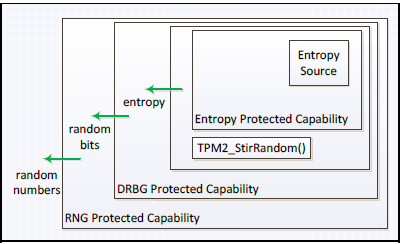
\includegraphics[scale=1]{Abbildung2.PNG} 
\captionof{figure}{Random Number Generation}
\label{fig:strukturvorlage}
\label{fig2}

\end{center}

\end{figure}

\subsubsection{Nonce Erstellung}

\section{Autorisations-Subsystem}
\section{Arbeitsspeicher (RAM)}
Direktzugriffsspeicher (RAM) enthält TPM-Transientendaten. Es ist zulässig, dass Daten im TPM-RAM verloren gehen, wenn die TPM-Stromversorgung unterbrochen wird. Da die Werte im TPM-RAM möglicherweise verloren gehen, werden sie in dieser Spezifikation als flüchtig bezeichnet, auch wenn der Datenverlust implementierungsabhängig ist.
Wenn sich die Spezifikation auf einen Wert bezieht, der sowohl flüchtige als auch nicht flüchtige Kopien aufweist, können sie an einem einzigen Ort aufbewahrt werden, solange dieser Ort die Eigenschaften des wahlfreien Zugriffs und der unbegrenzten Lebensdauer besitzt. \\
Nicht alle Werte im TPM-RAM befinden sich in abgeschirmten Positionen. Ein Teil des TPM-RAM enthält den E / A-Puffer mit Eigenschaften, die im Modul (I/O) beschrieben werden.
\subsection{Plattform-Konfigurationsregister (PCR)}
\subsection{Objektspeicher}
\subsection{Sessionsspeicher}
\subsection{Größenanforderungen}

\section{Nichtflüchtiger Speicher (NV-M)}
\section{TPM Operational States}
\section{Execution Engine}

\section{Leistungserkennungsmodul}
\section{Abschluss}

\section{Referenz}







